\section{Implementering af resultater}
Belønninger gives udfra samlet tid, afstand, antal træninger samt antal konditionstræninger og beregnes efter endt træning. Da disse belønninger er baseret ud fra den samlede træning, hentes den samlagte tid, afstand samt totale antal træninger fra databasen og omregnes til et tal mellem 1-6, der repræsenterer antallet af stjerner brugeren har opnået. Et udklip af javakoden for omregningen for brugere med en kategorisering "A" ses af \autoref{fig:kodebelon}.

\begin{figure} [H]
\centering
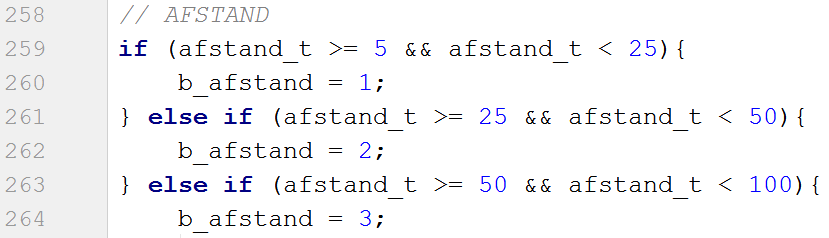
\includegraphics[width=0.8\textwidth]{figures/imple/kodebelon}
\caption{Udklip af javakode for omregning af samlet afstand til optjente belønninger for brugere med kategorisering "A".}
\label{fig:kodebelon}
\end{figure} 

\noindent
Det fremgår af dette javaudklip, at omregningen foregår ved hjælpe af if/else løkker. Hvis afstanden ligger indenfor et interval af 5 og 25 sættes \textit{b\_afstand} lig 1, hvilket repræsenterer én stjerne. Af \autoref{tab:SamletBelon} fremgår kriterierne for at opnå stjerner for brugere med kategoriseringen "A".  

\begin{table}[H]
\centering
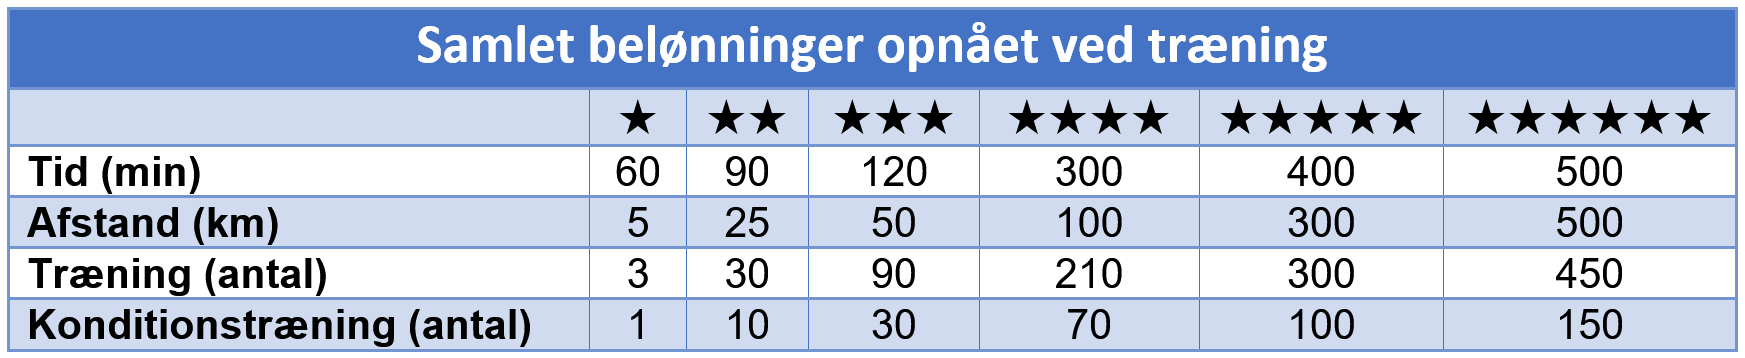
\includegraphics[width=0.8\textwidth]{figures/imple/SamletBelon}
\caption{Kriterier for at opnå belønninger inden for henholdsvis samlet tid, afstand og total antal træninger samt konditionstræninger for brugere med kategorisering "A".}
\label{tab:SamletBelon}
\end{table}  
